%-----------------------------------------------------------------------------%
%Packages%
\documentclass[12pt, a4paper, titlepage]{scrartcl}
\usepackage{amsmath, amsfonts, listings, amssymb, mathtools, amsthm} %Mathematical Expressions package
\usepackage{mathtools}
\usepackage[usenames, dvipsnames]{color} %Color naming packages
\usepackage[margin=1.5cm]{geometry}
\usepackage{float}
\usepackage{verbatim} %for code
\usepackage[pdftex]{graphics}
\usepackage{hyperref}
\usepackage{cleveref}
\usepackage{tikz}
\usepackage{comment}
\usepackage[nottoc]{tocbibind}
%\usepackage[square]{natbib}
\usepackage{caption}
\usepackage{subcaption}

\addtokomafont{disposition}{\rmfamily}
\usetikzlibrary{arrows,shapes}

%Graphis Extensions
\DeclareGraphicsExtensions{.png, .jpg}
\parindent 0pt

% Predefined things such as commands, etc.

\newcommand{\aRel}[1] {
  \sim_{#1} 
}

\newcommand{\kripkeFrame}[2] {
  (#1, \aRel{#2})
}

\newcommand{\kripkeModel}[3] {
  (#1, \aRel{#2}, #3)
}

\newcommand{\frKripModel}[2] { % defined via Kripke Frame + valuation
  (#1, #2)
}

\newcommand{\actModel}[3]{
  (#1, \aRel{#2}, #3)
}

\newcommand{\frActModel}[2] { % defined via Kripke Frame + Pre
  (#1, #2)
}

\newcommand{\note}[1]{\textsc{\textbf{#1}}}
\newcommand{\Universal}{$\mathcal{U}$}
\newcommand{\modalLog}{$\mathcal{L}$}
\newcommand{\modLogInf}{$\mathcal{L}_\inf$}
\newcommand{\epActLog}{\modalLog$([\alpha])$}
\newcommand{\epActLogCommonKnowledge}{\modalLog$([\alpha],\box^{*})$}

\newtheorem{defn}{Definition}
\newtheorem{thm}{Theorem}
\newtheorem{lemma}{Lemma}
\newtheorem*{remrk}{Remark}

% Drawings of frames

\tikzstyle{vertex}=[circle,fill=black!25,minimum size=20pt,inner sep=0pt]
\tikzstyle{selected vertex} = [vertex, fill=red!24]
\tikzstyle{edge} = [draw,thick,->]
\tikzstyle{weight} = [font=\small]

%-----------------------------------------------------------------------------%
%Document%
\begin{document}

\title{A Survey of Multi-agent Dynamic Epistemic Logic and Action Models}
\subtitle{UWA Final Year Engineering Project Literature Review}
\author{Edwin Tay, 20529864}
\date{\today}

\maketitle

\pagebreak

\tableofcontents

\vfill
\pagebreak

\section{Introduction}\label{intro}
\subsection{Describing Information State}\label{intro_infoState}
Multi-agent system are found in many fields, including communications systems,
artificial intelligence and games.
In part, multi-agent dynamic epistemic logic is concerned with modelling and reasoning
about what agents in these systems know.
This extends to how models are updated and what we can reason about agents'
perceptions of actions in a multi-agent system.
Being able to logically reason about what agents know and what actions they perceive
allows us to construct verifiable and correct specifications and claims about
models of situations.\\
\\
The change of agent knowledge via informative updates is a field that has seen
much attention recently.
Theorists have constructed models that capture these informative updates with
increasing expressiveness.
We discuss the increasing power and specificity of these models throughout this
survey, with a particular interest in public announcement logic in Section
\ref{pal} and epistemic actions and action models in Section \ref{estAct}. \\
\\
In a similar manner to models of knowledge, models of information updates can be
used to formally reason about updates.
The rigour of formalism is appealing for an application that aims to guarantee
security or verify that it fulfills a specification.
This formalism to formal, provable methods of software development,
communication protocol verification as well as economics and game theory.\\
\\
Recent work has focused on the synthesis of informative updates, showing how an
informative update can be constructed to ensure that, if possible, a multi-agent system
satisfies a condition after an update \cite{hales13synthesis}.
However, translating a formal model describing an informative update into an
implementation of communication between multiple agents is an unexplored
process.
Transforming a formally correct and verifiable specification of
communication into an executable protocol within a real world system would have
wide implications for software engineering, security and safety in
mission-critical systems with high-correctness requirements.
\subsection{A Game of Coins}\label{intro_coinFlipping}
Consider a game being played between two friends (or agents), Angeline $(A)$
and Ben $(B)$.
The game involves flipping a coin, hiding the result from both $A$ and $B$ and
having both of them guess whether the coin is Heads $(H)$ or the coin is Tails
$(T)$.
The game is refereed by a mutually trusted (and usually impartial) friend, Carol
$(C)$ who knows if the coin is $H$ or $T$.\\
\\
$A$ and $B$ know that either $H$ is true or $T$ is true.
They also know that $H$ and $T$ cannot both occur simultaneously together.
An agent's knowledge (which is inclusive of, but not limited to the previous
statements) is called the epistemic state.
Furthermore, there are two possibilities for the coin's outcome: that it is $H$
or $T$.
Neither $A$ or $B$ as they are can distinguish between them; that is, they are
uncertain which of the outcomes is true.
Agent uncertainty in this multi-agent system is another aspect we must attempt
to capture.\\
\\
This literature review considers the relevant writings and logics to describe
the epistemic state and how we can change and informatively update the epistemic
state.
The following sections will explore how we can model static situations and
different informative updates.
We will note what has not been explored in the fields and compare frameworks'
differing approaches and strengths.

\section{Epistemic Modal logic}\label{epistemic}
In the coin-flipping game, we can make the following observations.
\begin{itemize}
	\item $A$ considers $H$ to be possible, as well as $T$ to be possible
	\item $B$ also considers $H$ to be possible, and also considers $T$ to be possible
\end{itemize}
We claim that there are two possible worlds that differ in one way ---
in one of these worlds, $H$ is true, and in the other world $T$ is true.
Furthermore, these worlds are the same from $A$ and $B$'s perspectives.
$A$ would not be able to distinguish the world where $H$ was true from either of
the world where $H$ was true or the world where $T$ was true, since she cannot
see the coin.\\
\\
We can represent this uncertainty between what world is true as relations
between worlds.
In this case, let $W = \{ \eta, \tau\}$ be our set of possible worlds, where $H$ is true
at $\eta$ and $T$ is true at $\tau$.
Let $R_A = R_B = \{(\tau,\tau), (\tau,\eta), (\eta, \tau), (\eta,\eta)\}$ be
binary relations on $W$ representing indistinguishability between two possible
worlds.
We call these relations ``accessibility relations"; we say if one world is
indistinguishable from another, then they can access each other.
Lastly, let $V$ be a valuation function that maps a formula to the set of worlds
where that formula is true, so $V(H) = \{\eta\}$ and $V(T) = \{\tau\}$.
For a more formal, in-depth treatment of modal logic and the possible worlds model, see
texts by Blackburn, de Rijke and Venema \cite{blackburn2002modal} or van
Ditmarsch, van der Hoek and Kooi \cite{hoek2008dynamic}.
\begin{defn}
	The tuple
	\[
		M = (W, R = R_A \cup R_B, V)
	\]
	is an epistemic model of our game of heads and tails.
\end{defn}

We can represent this model graphically as shown in Figure \ref{htkripkefigure},
where our possible worlds $(W)$ are nodes and our binary relations $(R$) are edges in the
graph.
\begin{figure}[ht!]
\centering
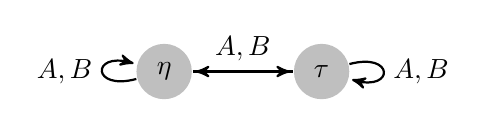
\begin{tikzpicture}[->,>=stealth',shorten >=1pt,auto,node distance=2cm,
      thick]

    \node[vertex] (1) {$\eta$};
    \node[vertex] (2) [right of=1] {$\tau$};
    \path[edge]
          (1) edge node {$A,B$} (2)
              edge [loop left] node {$A,B$} (1)
          (2) edge node {} (1)
              edge [loop right] node {$A,B$} (2);
\end{tikzpicture}
\caption{A graph representation of our game of heads and tails.}\label{htkripkefigure}
\end{figure}

The possible worlds models form a semantics allowing us to construct meaningful
models that reflect an epistemic state.
It is the semantics and models that allow us to reason about relations between the possible worlds in
an internal sense, from $A$ and $B$'s perspectives \cite{blackburn2002modal}.
We can define an operator to formally represent the modality of ``knowing"
a proposition or formula to be true.
\begin{defn}
	The operator $\Box_A H$ stands for ``$A$ knows $H$ is true".
	$\Box_A \phi$ is true at a possible world $w$ if for all accessibility relations $(w,
	w')$, $\phi$ is true.
\end{defn}
We also define the dual operator of knowing, which is to consider something
possible.
\begin{defn}
	The operator $\diamond_B T$ stands for ``$B$ considers $T$ to be possible".
	$\diamond_B \phi$ is true at a possible world $w$ if there is one
	accessibility relation $(w,w')$ such that $\phi$ is true at $w'$.\\
	
\end{defn}
\begin{note}
	N.B.: Notice that we can define $\diamond$ in terms of $\Box$, where $\diamond
	\phi \iff \neg \Box \neg \phi$.
\end{note}\\
\\
We will omit the name of the agent for operators $\Box$ and $\diamond$ when we
discuss a single-agent case, as follows.
We now show, without proof, four axioms that must hold for our modality of
knowledge.
\begin{thm}
	The following are true at any world of an epistemic model
	\cite{hoek2008dynamic}.
	\begin{enumerate}
		\item $\Box (\phi \implies \theta) \implies (\Box \phi \implies \Box
				\theta)$, known as {\bf K}
		\item $\Box \phi \implies \phi$, known as {\bf T}
		\item $\Box \phi \implies \Box \Box \phi$, labelled {\bf 4}
		\item $\neg \Box \phi \implies \Box (\neg \Box \phi))$, known as {\bf 5}
	\end{enumerate}
\end{thm}

\begin{note}
In order to satisfy these conditions, binary relations between possible worlds
in our epistemic models become equivalence relations.\\
\\
Also, if we replaced {\bf T} with an axiom {\bf D} which states $\Box \phi
\implies \diamond \phi$, then we can model Doxastic Models of belief, instead of
epistemic models of knowledge.
\end{note}\\
\\
We can now make formal reasonings, such as deciding that $\Box_A H$ and $\Box_A
T$ are both false.
We note that $\Box_B (H \lor T)$ is true and $\Box_A \Box_B (H \lor T)$ is
true.\\
\\
{\bf K}, {\bf T}, {\bf 4} and {\bf 5} allow us to model epistemic state and
uncertainty in our game of heads and tails.
We have defined on our models that allows us to make formal reasonings and
decide if formulae are true at possible worlds.\\
\\
But what if their friend, $C$, announces ``The coin is Heads up" (that is,
$C$ announces $H$)?
As they are, our models cannot describe the change in knowledge that
$C$'s announcement will entail.
Furthermore, we have no formal process to say how the situation has changed.\\
\\
This deficiency raises the following questions:
\begin{itemize}
	\item How do we describe this change in a formal manner?
	\item What reasoning can we make about the state of information after this
	change?
	\item Is there an operation that allows us to change the state of information
	from the pre-change state to the post-change state?
\end{itemize}

\section{Public Announcement logic}\label{pal}
To model the announcement of facts and information, we turn to the use of public
announcement logic.
Public announcements are announcements to multiple agents of facts.
They are a kind of informative update --- perhaps the most basic kind.\\
\\
Public announcement logic was first proposed independently by both Plaza and
Gerbrandy and Groeneveld \cite{plaza2007public,gelbrandy1997reasoning}.
They were later augmented by the work of Baltag, Moss and Solecki through the
addition of common knowledge \cite{baltag1998lpa}.
Public announcements are informational updates of true facts that change the
knowledge state amongst multiple agents.\\
\\
In the context of our card game, let us consider if our external trusted party
$C$ publicly announces to $A$ and $B$ that $H$ is true.
We will demonstrate the execution of that update upon our model in Figure
\ref{pakripkefigure}.
\begin{figure}[ht!]
\centering
\begin{subfigure}[b]{.45\textwidth}
\centering
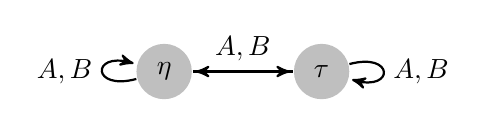
\begin{tikzpicture}[->,>=stealth',shorten >=1pt,auto,node distance=2cm,
      thick]

    \node[vertex] (1) {$\eta$};
    \node[vertex] (2) [right of=1] {$\tau$};
    \path[edge]
          (1) edge node {$A,B$} (2)
              edge [loop left] node {$A,B$} (1)
          (2) edge node {} (1)
              edge [loop right] node {$A,B$} (2);
\end{tikzpicture}
\caption{Our model before $H$ is announced to be true.}
\label{beforefigure}
\end{subfigure}
~
\begin{subfigure}[b]{.45\textwidth}
\centering
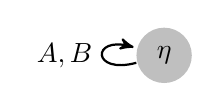
\begin{tikzpicture}[->,>=stealth',shorten >=1pt,auto,node distance=2cm,
      thick]

    \node[vertex] (1) {$\eta$};
    \path[edge]
          (1) edge [loop left] node {$A,B$} (1);
\end{tikzpicture}
\caption{Our model after $H$ is announced to be true.}
\label{afterfigure}
\end{subfigure}
\caption{The differences before and after the public announcements of $H$ to $A$ and
	$B$.}
\label{pakripkefigure}
\end{figure}
\\
Public announcements capture changes in information, such as $C$ saying to
$A$ and $B$ that the coin is $H$.
Another possible update is $A$ being allowed to see the coin's state, and
telling $B$ ``I guess you didn't know that the coin is actually heads up".\\
\\
These changes can be successful or unsuccessful, depending on whether the fact
that was announced is true after its announcement.
For example, if $A$ makes the (truthful) announcement that $H$, then this
announcement is successful since $H$ will be true after the announcement.\\
\\
Conversely, an announcement from $A$ to $B$ that ``I know that you {\em don't} know $H$
is true, but the coin is actually $H$".
We can write this as the announcement of the formula $H \land \neg \Box_B H$.
We can again refer to Figure \ref{pakripkefigure} to graphically show the models
before (Figure \ref{beforefigure}) and after (Figure \ref{afterfigure}) the update.
This update is interesting in that its announcement causes itself to be false.\\
\\
When $A$ publicly announces that the coin is $H$ and that $B$ does not know that
the coin is $H$ her announcement is now false, since $B$ now knows that $H$
actually is true.
Examining Figure \ref{afterfigure}, we can see that $H \land \neg \Box_B H$ is
untrue after its announcement in Figure \ref{beforefigure}.
This is an example of an unsuccessful public announcement.\\
\\
By using public announcement logic we can describe these announcements of
information.
We have a framework to describe and change the state of information amongst our
agents before and after announcements of facts.
Public announcement logic will allow us to model $C$ telling $A$ and $B$ in a
public fashion that $H$ is true.
This scales to modelling broadcasts in multi-agent systems, and allowing us to
update our models of the epistemic state of agents in such mass, public communications.\\
\\
In terms of dynamic epistemic logic, however, there could be many more kinds of
updates that we have yet to consider.
Re-examining our game of heads and tails yields scenarios that we cannot
describe:
\begin{itemize}
	\item What about $A$ cheating and learning $H$ or $T$ without $B$'s knowledge?
	\item What if $C$ was to whisper (in front of $B$) whether the coin was $H$
	or $T$?
\end{itemize}
These are things public announcement logic cannot describe, and our inability to
model them raises more questions:
\begin{itemize}
	\item what other kinds of epistemic (or informative) updates exist?
	\item how can we describe other epistemic updates in a sensible manner?
	\item what kind of an execution is required for a more nontrivial update?
\end{itemize}

\section{Epistemic Actions and Action Models} \label{estAct}
We can now successfully capture the simple act of announcing a fact.
However, in public announcements, we cannot capture certain updates to the
epistemic state, such as
\begin{itemize} 
  \item $C$ whispers to $A$ that $H$ is true and $B$ sees her whisper
  \item $C$ whispers to $A$ that $H$ is true without $B$ seeing
  \item $B$ suspects $A$ of cheating, but he isn't sure if she's cheated
\end{itemize}
Let us aim to generalise the ideas behind public announcements to capture other
informative updates.\\
\\
We will now constrain our agents' behaviours to only being able to accept facts.
They will not worry about changing facts, and if facts do change we will take it
as something that causes our agents knowledge systems to simply crash.\\
\\
We will examine two contrasting approaches to model these epistemic updates.
Our investigation will show the main differences in terms of what the frameworks
can describe and how we can use them to reason about updates.
\subsection{Epistemic Relational Actions} \label{epi_acts}
van Ditmarsch approaches epistemic actions from a syntactical point of view,
aiming to create a language to specify actions in.
His work in constructing an epistemic action syntax extends some of the
syntax of established languages such as propositional dynamic
logic\cite{ditmarsch99knowledge,ditmarsch2002dga}.\\
\\
van Ditmarsch provides operations to construct dynamic epistemic formulae, and
further extends the language with dynamic or action-oriented constructs.
These include the ability to test a proposition, to update a group of agents'
knowledge and to make a non-deterministic choice between actions.
Thus, van Ditmarsch presents a way to describe complex actions, and indeed we can
express and describe all the actions we've discussed in the previous sections.
We can formally describe actions such as cheating, or a private
announcement to $B$ that $H$ is true that's seen by $A$.\\
\\
However, reasoning about epistemic actions in their current form is difficult.
Indeed, the interpretations of an epistemic action are non-trivial to
understand.
Moreover, van Ditmarsch, van der Hoek and Kooi present problems with
representing complex uncertainties with van Ditmarsch's epistemic actions that make it difficult
to reason about what $A$ and $B$ know after an action takes place.\\
\\
In the next section, we review a different framework to model epistemic updates
which can describe as many updates as van Ditmarsch's language.
This framework resolves the issues with van Ditmarsch's epistemic actions and
has uncertainty about actions naturally encoded within it.
\subsection{Epistemic Action Models} \label{act_mods}
As an alternative to approaching epistemic actions syntactically, Baltag, Moss
and Solecki examine epistemic actions from a modelling point of view.
They aim to construct {\em epistemic action models}, which resemble the possible 
worlds models that were discussed in Section \ref{epistemic}
\cite{baltag1998lpa}.
Aucher resolves this into a possible actions model that allows us to make
reasonings about updates that are similar to reasonings about the epistemic
state.
This ``possible actions" model addresses the issues regarding reasoning about
actions and their outcomes using van Ditmarsch's framework, as discussed in
Section \ref{epi_acts} \cite{hoek2008dynamic}.\\
\\
We will consider the following situation, where our game of heads and tails
begins with both $A$ and $B$ unable to discern if the coin is $H$ or $T$ (Figure
\ref{ambeforefigure}).
However, $B$ leaves the room to use the bathroom and when he returns he is unable
to tell if $A$ has looked at the coin and learned that it is $H$, $T$ or whether
$A$ has not looked and nothing has changed \ref{amafterfigure}.
The graphical models for each situation are presented in Figure
\ref{amkripkefigure}.\\

\begin{figure}[ht!]
\centering
\begin{subfigure}[b]{.45\textwidth}
\centering
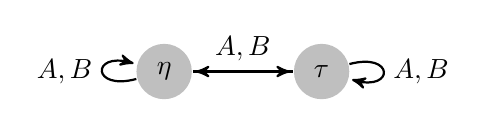
\begin{tikzpicture}[->,>=stealth',shorten >=1pt,auto,node distance=2cm,
      thick]

    \node[vertex] (1) {$\eta$};
    \node[vertex] (2) [right of=1] {$\tau$};
    \path[edge]
          (1) edge node {$A,B$} (2)
              edge [loop left] node {$A,B$} (1)
          (2) edge node {} (1)
              edge [loop right] node {$A,B$} (2);
\end{tikzpicture}
\caption{Our model before $B$ temporarily left the game.}
\label{ambeforefigure}
\end{subfigure}
~
\begin{subfigure}[b]{.45\textwidth}
\centering
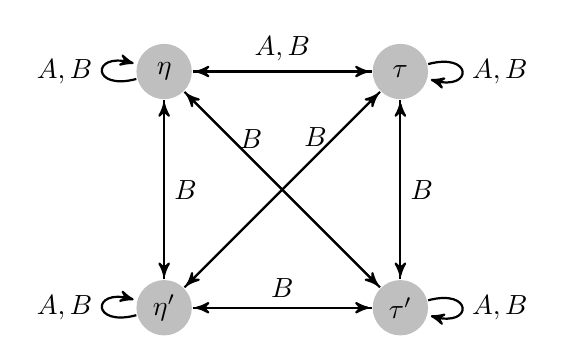
\begin{tikzpicture}[->,>=stealth',shorten >=1pt,auto,node distance=3cm,
      thick]

    \node[vertex] (1) {$\eta$};
    \node[vertex] (2) [right of=1] {$\tau$};
    \node[vertex] (3) [below of=1] {$\eta'$};
    \node[vertex] (4) [right of=3] {$\tau'$};
    \path[edge]
          (1) edge node {$A,B$} (2)
              edge [loop left] node {$A,B$} (1)
							edge node {$B$} (3)
							edge node {} (4)
          (2) edge node {} (1)
              edge [loop right] node {$A,B$} (2)
							edge node [above,pos = 0.33] {$B$} (3)
							edge node {$B$} (4)
					(3) edge node {} (1)
							edge node {} (2)
							edge node {$B$} (4)
							edge [loop left] node {$A,B$} (3)
					(4) edge node [above, pos = 0.66] {$B$} (1)
							edge node {} (2)
							edge node {} (3)
							edge [loop right] node {$A,B$} (4);
\end{tikzpicture}
\caption{Our model after $B$ returns and is unsure about whether $A$ has looked
	at the coin.
$\tau$ and $\eta$ are worlds where $A$ has not cheated while $\tau'$ and $\eta'$
are worlds where $A$ has cheated and looked at the coin.}
\label{amafterfigure}
\end{subfigure}
\caption{The differences before and after $B$'s temporary departure.}
\label{amkripkefigure}
\end{figure}

In Figure \ref{amkripkefigure}, we can say that $H$ is true at $\{\eta,\eta'\}$ and $T$ is
true at $\{\tau,\tau'\}$, but that in $\eta'$ and $\tau'$ $A$ has taken a look
at the coin and can distinguish between $\eta'$ and $\tau'$.
Our change in epistemic state is a change that we cannot model with public
announcement logic.
It is a private announcement such that $B$ is aware of the announcement, but not
of its contents.\\
\\
This update is one we can capture with an action model.
$B$ considers it possible that an action where $A$ looks at the coin and learns
$H$ occurs.
He also considers the action where $A$ looks at the coin and learns $T$ possible
as well.
Lastly, he considers that $A$ did not look at the coin and thus the state of the
world remains the same, signified by {\bf tr}.
As $B$ cannot tell which one of them occurred, but is aware that one of them did
occur, he considers them indistinguishable.
We can represent them as a ``possible actions" model, as we show in Figure
\ref{amprivatea}.
Baltag, Moss and Solecki define an operation to execute the model in Figure
\ref{amprivatea} on Figure \ref{ambeforefigure}, yielding Figure
\ref{amafterfigure}\cite{baltag1998lpa}.

\begin{figure}[H]
\centering
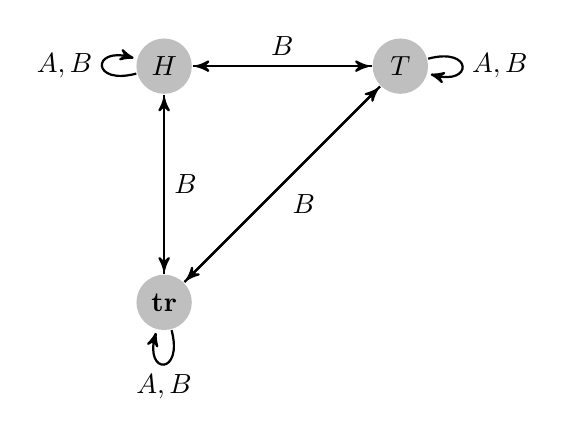
\begin{tikzpicture}[->,>=stealth',shorten >=1pt,auto,node distance=3cm,
      thick]

    \node[vertex] (1) {$H$};
    \node[vertex] (2) [right of=1] {$T$};
    \node[vertex] (3) [below of=1] {{\bf tr}};
    \path[edge]
          (1) edge node {$B$} (2)
							edge node {$B$} (3)
              edge [loop left] node {$A,B$} (1)
          (2) edge node {} (1)
							edge node {$B$} (3)
              edge [loop right] node {$A,B$} (2)
					(3) edge [loop below] node {$A,B$} (3)
							edge node {} (1)
							edge node {} (2);
\end{tikzpicture}
\caption{An example of an action model; in this example, the update models $B$
becoming suspicious of $A$ having learnt whether $H$ or $T$ is true, but not
knowing whether the $A$ actually has not learnt anything and the world remains
as it was before (signified {\bf tr}).}
\label{amprivatea}
\end{figure}

Baltag and Moss extend the action models they proposed with Solecki into classes
of action models, which they term action signatures \cite{baltag2005programs}.
They formalise general descriptions of actions, such as announcements, private
announcements, lying, suspicion and other epistemic updates.
As an example, they generalise all public announcements to a single structure,
showing the superior expressiveness of action models.
They also specify a syntax for discussing actions of a given action signature,
allowing them to generate the logic of public announcements in its entirety.
Within this syntax, the action model structures are used as syntactical objects.
Like van Ditmarsch's epistemic actions, Baltag and Moss' syntax extends previous
logics of dynamics and change.\\
\\
Action models are define a method of execution upon an epistemic model that is well-understood.
The execution will update a model of knowledge from a pre-update to a
post-update state.
Unfortunately, the cost of action model execution (that is, to transform a state
of information to a new state using an update specified by an action model) is
quite high.
It involves taking a Cartesian product of all possible actions.
This indicates that, given $N$ possible actions in an action model, $N^2$
actions must be computed in the new state of information before the model can
be refined.

\subsubsection{Comparison to relational epistemic actions} \label{epi_compare}
Both relational epistemic actions \cite{hoek2008dynamic} and action models
\cite{baltag1998lpa} describe a larger range of epistemic updates for our game of heads and tails.
The examples we chose earlier, regarding $C$ telling $A$ about the state of the
coin, or $B$ becoming suspicious of $A$ can be expressed using either framework.
What, then, is the real difference between employing action models, as opposed
to relational epistemic actions?\\
\\
van Ditmarsch, van der Hoek and Kooi, as well as Baltag and Moss independently
note that the ``possible actions" of action models  are actually relational
epistemic actions.
In their own review of action models, van Ditmarsch, van der Hoek and Kooi
motivate this with an example \cite{hoek2008dynamic,baltag2005programs}.\\
\\
They consider the non-deterministic choice of 3 possible actions which are
indistinguishable externally.
As an example, $B$ might learn that $A$ knows either of $H$ or $T$, or has
learnt nothing at all.
Since $B$ does not know which of these actions could occur, each of these
epistemic updates is a possible action.\\
\\
They show that it is possible to express this uncertainty in a manner quite similar
to an action model.
Similarly, the corresponding action model of whether $B$ learns of $A$'s
knowledge of $H$, $T$ or nothing new is quite easily interpreted in a manner
akin to relational epistemic actions.
Their general result is that relational actions can be expressed as action
models, and vice versa.
As van Ditmarsch, van der Hoek and Kooi have already shown, it is in reasoning
with these models that the models differ.\\
\\
Notably, relational epistemic actions and action models suffer from the same
weakness, in that they are only externally describe an update of information.
Their execution and specification are only useful to a third-party viewer, and
how agents internal to a system update their knowledge is not clear.
This is one of several weaknesses in current dynamic epistemic logic, with
regards to translating a specification of an informational update into an
implementable series of messages.\\
\\
It is in their reasoning that action models and relational epistemic actions
differ most.
action models give us a notion of uncertainty between actions in a manner
similar to the possible worlds model, allowing us to use a formally established framework
to reason about dynamic updates.
This allows us to reason about our updates and their effects in a more natural
and well-understood way.\\
\\
Conversely, van Ditmarsch's relational epistemic actions give us a syntax that
is perhaps more natural than the one Baltag and Moss define.
Baltag and Moss are note that it is non-standard to use the modelling structures
inside a syntax \cite{baltag2005programs}.
In the context of interpreting and making sensible updates, however, it is
perhaps less useful to have abstraction at the cost of useful interpretations,
suggesting that action models are a more interesting way to model epistemic
updates.
Indeed, it would appear that at the moment action models are experiencing more
interest compared to relational epistemic actions, as we explore in the next
section.

\subsection{Extensions of action models}
Action models, when first introduced, were a concept that could be used to make
formal reasonings about actions in a similar way to possible worlds semantics.
Progress in this area has added a syntax that uses action models as syntactic
objects, improved the expressiveness of action models and investigated the
synthesis of action models.
Much of the discussion has showed how powerful action models are as a way for a
third party to reason about an informational update, and improved what kind of
informational updates we can capture.\\
\\
Baltag and Moss define a powerful syntax for constructing epistemic programs.
Their syntax is as powerful as van Ditmarsch's in relational epistemic actions,
being able to express sequences of epistemic actions or make a non-deterministic
choice between two established action models.
In our game, we would be able to model sequences of actions, such as $A$ finding
out whether $H$ is true or $T$ is true while $B$ watches, then $B$ finding out
whether $H$ or $T$ is true but without $A$ being aware of $B$ learning this \cite{baltag2005programs}.\\
\\
The only objection to their syntax, as raised earlier, is the curious use of
the semantic structures within a syntax.
It is also notable that the operations of composition and non-deterministic
choice can be as costly as action model execution, generating $N \times M$
possible actions, given two action models of size $N$ and $M$
respectively \cite{baltag2005programs}.\\
\\
van Benthem, van Eijck and Kooi extend action models for a new language to
handle communication and change.
Their main contribution here is to improve action model languages with notions
of group knowledge and iterations of an action model's execution.
This logic of communication and change uses previous logics of change as a basis
and proceeds to interpret it in an epistemic fashion\cite{benthem2006lcc}.\\
\\
van Ditmarsch, French and Pinchinat construct a future action model logic in
their contribution.
Together, their work shows how one can determine if for a particular possible
world it is possible to update it such that a condition $\phi$ is true after an
update \cite{van2009simulation,van2010future}.\\
\\
In a recent contribution, Hales describes an algorithm that can synthesise arbitrary
action models.
Hales builds upon van Ditmarsch and French's work, showing that if an action
model $\alpha$ exists to ensure a condition $\phi$ was true after that models
execution, then there is a method by which an equivalent action model can be generated.
This contribution is especially notable due to it generalising outside of
epistemic logic, to any modal logic system.
Thus it is possible to transform any modal logic model into another modal logic
model using action models\cite{hales13synthesis}.\\
\\
This shows that we can use action models to ensure a condition is true
in a new epistemic state, if it is at all possible.
As an example, if in our game of coins $A$ and $B$ are unsure whether $H$ or $T$
are true, we would be able to determine if an action model exists that could
make it so that after its execution, $\Box_A H \land \Box_B H$ was true at a
specific world.
Hales' work would allow us to synthesise this action model.\\
\\
The state of the art in action models and this section of dynamic epistemic
logic is thus focused upon improving descriptions of information updates, or how
we can use them to achieve a given epistemic state.
None of this research discusses how an action model can be implemented in a
real-world system.
Instead, action models have become better at describing changes, but how they
should be implemented is still unclear.

\subsubsection{Future Work}
Whilst the expressiveness and operators in languages involving action models are
improving (as in \cite{benthem2006lcc}) action models are treated as purely
descriptive objects.
We note two avenues of research that, as of yet, do not appear to have been
investigated.
\begin{enumerate}
	\item action models are external descriptions in their nature; they are only used as
	descriptions, so how an agent who is participating in the communications
	should use them is unclear
	\item action models have not been translated into real-world systems and no
	known method exists to change an action model into an implemented sequence of
	messages. The actual cost of action model execution in a real-world system has
	never been measured due to no-one ever implementing an action model.
\end{enumerate}
Thus, action models only describe changes, and the execution and expense
of their execution (whether in terms of time, size of intermediate models or
complexity) is not taken into account.
This makes it less clear how useful an action model would be, without a method
of transforming a description into an implementation.\\
\\
Perhaps the closest related work regarding the expense of an update might be
Bollig et. al's findings regarding communications and message passing with
dynamic logics.
The dynamic logics they utilise in their work are the same as those that van
Benthem et. al base their own work upon.
Their findings show that message passing sequences need to be of exponential
length in order to capture logical statements \cite{bollig07mps}.\\
\\
However, Bollig et. al approach message passing from the perspective of dynamic
logic.
Although van Benthem et. al use the same dynamic logic in their system, the
programs and information updates that they aim to capture might be more specific
than the general cases Bollig et. al appear to be interested in.
Thus, even though it is for a message passing sequence, there may be
structures of action models specifically that we can capture.\\
%\\
%As it stands, Bollig et. al's research is tangential to the work of van Benthem
%et. al.
%With regards to action models, the work thus far is confined to being only
%useful for expressing specification of change, and whether or not such
%specification implemented remains to be seen.\\
\\
van Benthem et. al also note that they had not interested themselves with methods of
generating action models from an ``atomic" set of Action
Models\cite{benthem2006lcc}.
They lay out their intuitions about how to generate action models and the class
of epistemic updates, but decide not to investigate this avenue of enquiry.
This presents another unexplored avenue regarding action models' generation from
an atomic set of action models, as well as what these atomic sets are.\\
\\
Thus, although action models are appropriate for descriptions there is not
method to take an action model and transform it into an implementation.
In addition to the two areas of further investigation that we noted at the
beginning of this section, we now observe a third area for further work.
That is, it is unclear how we could generate all action models from a
set of atomic action models.

\section{Conclusion} \label{conc}
We have displayed logics that have become progressively more expressive,
motivating their usage with the epistemic state of a multi-agent coin game.
This survey has identified three open problems where further investigation could contribute towards
transforming action models from models of epistemic updates into realisable
implementations.
\begin{enumerate}
	\item action models are descriptive and useful for external modelling --- how
	they are useful internally for agents involved in a multi-agent system is
	unclear
	\item How an action model can be translated from a theoretical ``possible
	actions" models into a sequence of messages to realise execution in a
	real-world multi-agent system remains to be seen
	\item Little work has been done into how to generate all action models from
	an atomic set of action models and what those Actions would be
\end{enumerate}

\bibliographystyle{ieeetr}
\bibliography{litReview}

\end{document}
